% % % % % % % % % % % % % % % % % % % % % % % % % % % % % % % % % % % % % % % % 
% Formelsammlung von LaTeX4EI									
%
% @encode: 	UTF-8, tabwidth = 4, newline = LF
% @author:	Lukas Kompatscher
% @date:	18.03.2016	
%
% % % % % % % % % % % % % % % % % % % % % % % % % % % % % % % % % % % % % % % % 

%---------------------------------------%
%				Analysis 3				%
%~~~~~~~~~~~~~~~~~~~~~~~~~~~~~~~~~~~~~~~%

% Document Class ===============================================================
\documentclass[german,color,5pt]{latex4ei_fs}

% set document information
\title{Analysis 3}
\author{Lukas Kompatscher und Roberto Gudelj}	
\myemail{lukas.kompatscher@tum.de}	

\DeclareTextFontCommand{\emph}{\bfseries}
\titleformat{\subsubsection}{\normalsize\bfseries}{\thesubsubsection.\ }{0pt}{}

% Redefine \i to produce an upright imaginary unit
\renewcommand{\i}{\mathrm{i}}


% DOCUMENT_BEGIN ===============================================================
\begin{document}

\maketitle

% SECTION ======================================================================
\section{Nützliches Wissen \quad $e^{\i x} = \cos (x) + \i \cdot \sin(x)$}
% ==============================================================================
\begin{sectionbox}
	\subsection{Sinus, Cosinus \quad $\sin^2(x) \bs + \cos^2(x) = 1$}
	$ \sin x = \frac{1}{2\i}(e^{\i x}-e^{-\i x}) \qquad \quad \cos x = \frac{1}{2}(e^{\i x}+e^{-\i x})$
	\begin{tablebox}{c|c|c|c|c||c|c|c|c}
	$x$ & $0$ & $\pi / 6$ & $\pi / 4$ & $\pi / 3$ & $\frac{1}{2}\pi$ & $\pi$ & $1\frac{1}{2}\pi$ & $2 \pi$ \\
	%$\scriptstyle{ \varphi }$ & $\scriptstyle{0^\circ}$ & $\scriptstyle{30^\circ}$ & $\scriptstyle{45^\circ}$ & $\scriptstyle{60^\circ}$ & $\scriptstyle{90^\circ}$ & $\scriptstyle{180^\circ}$ & $\scriptstyle{270^\circ}$ & $\scriptstyle{360^\circ}$ \\
	\cmrule
	$\sin$ & $0$ & $\frac{1}{2}$ & $\frac{1}{\sqrt{2}}$ & $\frac{\sqrt 3}{2}$ & $1$ & $0$ & $-1$ & $0$ \\
	$\cos$ & $1$ & $\frac{\sqrt 3}{2}$ & $\frac{1}{\sqrt 2}$ & $\frac{1}{2}$ & $0$ & $-1$ & $0$ & $1$ \\     
	$\tan$ & $0$ & $\frac{\sqrt{3}}{3}$ &	$1$	&	$\sqrt{3}$ & $\pm \infty$ & $0$ & $\mp \infty$ & $0$\\ 
	\end{tablebox}
	\begin{tablebox}{ll}
		Additionstheoreme &  Stammfunktionen\\
	 	$\cos (x - \frac{\pi}{2}) = \sin x$ & $\int x \cos(a x) \diff x = \frac{a x \sin(a x)+\cos(a x)}{a^2}$\\
	 	$\sin (x + \frac{\pi}{2}) = \cos x$ & $\int x \sin(a x) \diff x = \frac{\sin(a x)-ax\cos(a x)}{a^2}$\\
	 	$\sin 2x = 2 \sin x \cos x $  & $\int \sin^2(ax) \diff x = \frac{x}{2}-\frac{\sin(2ax)}{4a}$\\ 
	 	$\cos 2x = 2\cos^2 x - 1$  & $\int \cos^2(ax) \diff x = \frac{x}{2}+\frac{\sin(2ax)}{4a}$\\
	 	$\tan(x) = \frac{\sin(x)}{\cos(x)}$ & $\int \cos(x)\sin(x) = -\frac12 \cos^2(x)$ \\
	 	
	 	%Spezialfälle
	 	% $\int x \cos(x) \diff x = \cos(x) + x \sin(x)$\\
		% $\int x \sin(x) \diff x = \sin(x) - x \cos(x)$
		% $\int \sin^2(x) \diff x = \frac12 \bigl(x - \sin(x)\cos(x) \bigr)$
		% $\int \cos^2(x) \diff x = \frac12 \bigl(x + \sin(x)\cos(x) \bigr)$
	 	
	 	\multicolumn{2}{l}{\!\!\!\!\!\! $\sin ( x \pm y ) = \sin x \; \cos y \pm \cos x \; \sin y$} \\
	 	\multicolumn{2}{l}{\!\!\!\!\!\! $\cos ( x \pm y ) = \cos x \; \cos y \mp \sin x \; \sin y$} \\
	 	
	\end{tablebox}
		\textbf{Sinus/Cosinus Hyperbolicus}\\ 
		% \quad \operatorname{arsinh}\ x:= \ln\left(x+\sqrt{x^2+1}\right) \\
		\begin{tabular*}{\columnwidth}{@{\extracolsep\fill}ll@{}}
		$\sinh x = \frac{1}{2}(e^x -e^{-x})= - \i \, \sin(\i x)$ & $\cosh^2 x  \bs - \sinh^2 x = 1$\\
		$\cosh x  = \frac{1}{2}(e^x +e^{-x})= \cos(\i x)$ & $\cosh x + \sinh x = e^{x}$\\
		\end{tabular*}\\
		\textbf{Kardinalsinus} $\mathrm{si}(x) = \frac{\sin(x)}{x}$ \qquad genormt: $\sinc(x) = \frac{\sin(\pi x)}{\pi x}$
\end{sectionbox}

\begin{sectionbox}
	\subsection{Integrale $\int e^x\;\mathrm{d} x = e^x = (e^x)'$}
	Partielle Integration: $\int uw'=uw-\int u'w$\\
	Substitution:  $\int f(\underbrace {g(x)}_{t}) \underbrace {g'(x)\,\mathrm dx}_{\mathrm dt}=\int f(t)\, \mathrm dt$
	\renewcommand{\arraystretch}{1.6} 
	\begin{tablebox}{ccc}
		$F(x)$ & $f(x)$ & $f'(x)$ \\ \cmrule
		$\frac{1}{q+1}x^{q+1}$ & $x^q$ & $qx^{q-1}$ \\
		\raisebox{-0.2em}{$\frac{2\sqrt{ax^3}}{3}$} & $\sqrt{ax}$ & \raisebox{0.2em}{$\frac{a}{2\sqrt{ax}}$}\\
		$x\ln(ax) -x$ & $\ln(ax)$ & $\textstyle \frac{a}{x}$\\
		%e^x & e^x & e^x \\
		$\frac{1}{a^2} e^{ax}(ax- 1)$ & $x \cdot e^{ax}$ & $e^{ax}(ax+1)$ \\
		$\frac{a^x}{\ln(a)}$ & $a^x$ & $a^x \ln(a)$ \\
		$-\cos(x)$ & $\sin(x)$ & $\cos(x)$\\
		$\cosh(x)$ & $\sinh(x)$ & $\cosh(x)$\\
		$-\ln |\cos(x)|$ & $\tan(x)$ & $\frac{1}{\cos^2(x)}$ \\
	\end{tablebox}
	
	$\int e^{at} \sin(bt) \diff t = e^{at} \frac{a \sin(bt) - b \cos(bt)}{a^2 + b^2}$ \qquad $x=\frac{-b\pm \sqrt{b^2-4ac}}{2a}$ \\
	\begin{tablebox}{ll}
		$\int \frac{1}{\sqrt{at+b}} \diff t = \frac{2 \sqrt{at+b}}{a}$ & $\int t^2 e^{at} \diff t = \frac{(at-1)^2+1}{a^3} e^{at}$\\
		$\int t e^{at} \diff t = \frac{at-1}{a^2} e^{at}$ & $\int x e^{ax^2} \diff x = \frac{1}{2a} e^{ax^2}$\\
	\end{tablebox}
\end{sectionbox}

\begin{sectionbox}
	\subsection{Exponentialfunktion und Logarithmus $k\in\mathbb{Z}$}
	\begin{tabular}{lll}
		$a^x = e^{x \ln a}$ & $\log_a x = \frac{\ln x}{\ln a}$ & $\ln x \le x -1$\\
		$\ln(x^{a}) = a \ln(x)$ & $\ln(\frac{x}{a}) = \ln x - \ln a$ & $\log(1) = 0$\\
		$e^0=e^{\i2\pi k}=1$ & $e^{\i\pi k} =(-1)^k$ &  $e^{\i \frac{\pi}{2} k} =\i^k$ 
	\end{tabular}
\end{sectionbox}

\begin{sectionbox}
	\subsection{Betrag komplexer Zahlen und komplexe Wurzel}
	$\abs{\cx z}^2 = \cx z \cxc z = x^2+y^2$ \\
	 $\sqrt[n]{\cx z}=\sqrt[n]{|\cx z|} \exp \left( \frac{\i \varphi}{n} + k\frac{2\pi\i}{n}\right)$ mit $k=0,\dots,n-1$
\end{sectionbox}

\begin{sectionbox}
	\subsection{Reihen}
	$\underset{\text{Harmonische Reihe}}{\sum\limits_{n=1}^\infty \frac{1}{n} \ra \infty} \qquad   \underset{\text{Geometrische Reihe}}{\sum\limits_{n=0}^\infty z^n \stackrel{|z|<1}= \frac{1}{1-z}}  \qquad \underset{\text{Exponentialreihe}}{\sum\limits_{n = 0}^{\infty} \frac{z^n}{n!} = e^z}$
\end{sectionbox}

%UNWICHTIG
%\begin{sectionbox}
%	\subsection{Wichtige Formeln}
%	%noneed \setlength{\tabcolsep}{0pt}
%	
%	\begin{tablebox}{ll}
%			Dreiecksungleichung: &$\big|\! \abs{x}- \abs{y}\!\big| \le \abs{x \pm y} \le \abs{x} + \abs{y}$\\
%			Cauchy-Schwarz-Ungleichung: & $\left| \vec x^\top \bdot \vec y \right| \le \| \vec x\| \cdot \| \vec y\|$ \\
%			Bernoulli-Ungleichung: & $(1+x)^n \ge 1+nx$\\ \cmrule
%			Aritmetrische Summenformel &  $\sum \limits_{k=1}^{n} k = \frac{n (n+1)}{2} $ \\
%			Geometrische Summenformel &  $ \sum \limits_{k=0}^{n} q^k = \frac{1 - q^{n+1}}{1-q}$ \\
%			Binomialkoeffizient & $\binom nk = \binom n{n-k} = \frac{n!}{k! \cdot (n-k)!}$\\
%	\end{tablebox}
%\end{sectionbox}
	

% SECTION ======================================================================
\section{Fourierreihe \quad $f(x) \sim F(x)$ \qquad $\omega = \frac{2 \pi}{T}$}
% ==============================================================================
\begin{sectionbox}
	\emph{Voraussetzungen:}
	\begin{enumerate}
		\item $f$ ist $T$-periodisch im Intervall $I$, meist $I=[-\frac{T}{2},\frac{T}{2})$ oder $I=[0,T)$
		\item $I$ aufteilbar in Teilintervalle, in denen $f$ stetig und monoton
		\item In den endlich viele Unstetigkeitsstellen existieren links- und rechtsseitige Grenzwerte
	\end{enumerate}
	$f$ ist $T$-periodisch, falls $f(x+T) = f(x)$ $\Ra$ auch $n \cdot T$ periodisch.\\\\
	\textbf{Reelle Fourierreihe:}
	\begin{emphbox}\vspace{-5pt}
		\[F(x) = \frac{a_0}{2} + \sum\limits_{k=1}^\infty a_k \cos \left(k \omega x \right) + b_k \sin \left( k \omega x \right)\]
		\[\text{mit } a_k,b_k \in \R \text{(bzw. } \C\text{)}:\Big\{ { ^{\textstyle a_k}_{\textstyle b_k}} = \frac{2}{T} \int\limits_{-\frac{T}{2}}^{\frac{T}{2}} f(x) \Big\{ {}^{\textstyle \cos} _{\textstyle \sin} \left(k \omega x \right) \diff x\]
	\end{emphbox}
	$a_0$ immer separat berechnen mit $k=0$\\
	\textbf{Komplexe Fourierreihe:}
	\begin{emphbox}\vspace{-5pt}
		\[F(x) = \sum\limits_{k=-\infty}^\infty c_k \exp \left( \i k \omega x \right)\]
		\[\text{mit } c_k \in \C: c_k = \frac{1}{T} \int\limits_{-\frac{T}{2}}^{\frac{T}{2}} f(x) \exp \left( - \i k \omega x \right) \diff x\]
	\end{emphbox}	
	$c_0$ immer separat berechnen mit $k=0$\\
	\emph{Konvergenz:} $F(x) \sim f(x)$
	\begin{itemize}
		\item $f$ in $x$ \emph{stetig \& stückweise stetig differenzierbar} $\Ra$ $F(x) = f(x)$
		\item $f$ in $x$ \emph{nicht stetig} $\Ra$ $x = a_i$ und $F(x) = \frac{f(a_i^+) + f(a_i^-)}{2}$
	\end{itemize}
\end{sectionbox}

\begin{sectionbox}
	\subsection{Rechenregeln}
	\begin{tablebox}{ll}
		Linearität & $\alpha f + \beta g \T \alpha c_k + \beta d_k$\\
		Konjugation & $\ol{f} \T \ol{c_{-k}}$\\
		Zeitumkehr & $f(-t) \T c_{-k}$\\
		Streckung & $f(\gamma t) \T c_k; \gamma > 0; \tilde{T} = \frac{T}{\gamma} \Leftrightarrow \tilde \omega = \gamma \omega$\\
		Verschiebung $t$ & $f(t + a) \T e^{\i k \omega a} c_k$\\
		Verschiebung $\omega$ & $e^{\i n \omega t} f(t) \T c_{k - n}$\\
		Ableitung & $\dot{f}(t) \T \i k \omega c_k$\\
		Ableitung bei Sprungstellen & $\dot{f}(t) \T \i k\omega c_k - \frac{1}{T}\sum_{j=1}^{N}\Delta_j e^{-k\omega tj}$\\
		Stammfunktion & $\int_0^t f(t) \T \begin{cases} \frac{c_k}{\i k \omega} & k \neq 0\\ -\frac{1}{T}\int_0^T t f(t) \diff t & k = 0\\ \end{cases}$\\
		& $c_{0_{f(t)}} \stackrel{!}{=} 0$\\
		Faltung & $f * g \T c_k d_k$\\
	\end{tablebox}
\end{sectionbox}

\begin{sectionbox}
	\subsection{Symmetrien}
	\begin{itemize}
		\item $f$ gerade (achsensym.) Funktion: $f(t) = f(-t)$\\
		$c_k = c_{-k}$\\
		$b_k = 0$ \qquad $a_k = \frac{4}{T} \int_{0}^{T/2} f(x) \cos \left(k \omega x \right) \diff x$
		\item $f$ ungerade (punktsym.) Funktion: $f(t) = -f(-t)$\\
		$c_k = -c_{-k}$\\
		$a_k = 0$ \qquad $ b_k = \frac{4}{T} \int_{0}^{T/2} f(x) \sin \left(k \omega x \right) \diff x$
		\item $f$ $\frac{T}{2}$-periodisch: $f(\frac{T}{2} + t) = f(t)$\\
		$c_{2k+1} = a_{2k+1} = b_{2k+1} = 0$\\
		$\begin{cases} a_{2k}\\ b_{2k} \end{cases} = \frac{1}{T}\int_0^{T/2}f(t)\begin{cases} \cos{(2k \omega t)}\\ \sin{(2k \omega t)} \end{cases} \diff t$
		\item $f$ ohne $\frac{T}{2}$-periodischen Anteil: $f(\frac{T}{2} + t) = -f(t)$\\
		$c_{2k} = a_{2k} = b_{2k} = 0$\\
		$\begin{cases} a_{2k+1}\\ b_{2k+1} \end{cases} = \frac{1}{T}\int_0^{T/2}f(t)\begin{cases} \cos{((2k+1) \omega t)}\\ \sin{((2k+1) \omega t)} \end{cases} \diff t$
	\end{itemize}
\end{sectionbox}

\begin{sectionbox}
	\subsection{Umrechnungsformeln}
	\begin{itemize}
		\item $a_0 = 2 c_0 \quad a_k = c_k + c_{-k}$  \quad $b_k = \i (c_k - c_{-k})$
		\item $c_0 = \frac{a_0}{2} \quad c_k = \frac12(a_k - \i b_k) \quad c_{-k} = \frac12(a_k + \i b_k)$
	\end{itemize}
\end{sectionbox}

\begin{sectionbox}
	\subsection{Umrechnung von $T$ in $S$ periodische Funktionen}
	$f$ ist $T$ periodisch, $g(x) = f\left( \frac{T}{S} x \right)$, $S$ periodisch, denn
	$g(x+S) = f\left( \frac{T}{S} (x+S) \right) = f\left( \frac{T}{S} x + T \right) = f\left( \frac{T}{S} x \right) = g(x)$\\
\end{sectionbox}

\begin{sectionbox}
	\subsection{LTI-Systeme ($c_k$ sind Fourierkoeffizienten von $x(t)$) }
	$L[y](t) = a_n y^{(n)}(t) + \cdots + a_1 \dot{y}(t) + a_0 y(t) = x(t)$\\
	$\frac{\diff^n}{\diff t^n} \ra s^n \Ra P(s) = a_n s^n \cdots + a_1 s + a_0$\\
	$h_T(t) = \sum_{k=-\infty}^{\infty}d_k e^{\i k \omega t}$ mit $d_k = \frac{1}{P(\i k \omega)}$\\
	$y(t) = h_T(t)*x(t) = \int_0^T h_T(\tau) x(t - \tau) \diff \tau = \sum c_k d_k e^{\i k\omega t}$
	
\end{sectionbox}

\begin{sectionbox}
	\subsection{Funktionen}
	\subsubsection{Sägezahnfunktion}
	$s(t) = \frac{1}{2}(\pi - t), \quad 0 < t < 2 \pi, \quad T = 2 \pi, \quad \omega = 1$\\
	$c_0 = 0 \qquad c_{k\ne 0} = \frac{1}{2k \i}$ \quad bzw. \quad $ a_0 = 0 \qquad a_k=0 \qquad b_k=\frac{1}{k}$\\
	$S(t) = \sum_{k=1}^{\infty}\frac{1}{k}\frac{e^{\i k t} - e^{-\i k t}}{2 \i} = \sum_{k\ne 0}\frac{1}{2\i k}e^{\i k t}$
	\subsubsection{Weiterer Sägezahn, Rechteck und Treppenfunktion ($2\pi$-periodisch)}
	\begin{tablebox}{ll}
		$f:[-\pi,\pi) \ra \mathbb{R}, f(x)=x$ & $a_k=0, b_k=\frac{2}{k}(-1)^{k+1}$ \\
		$f:[-\pi,\pi) \ra \mathbb{R}, f(x)=\operatorname{sgn}(x)$ & $a_k=0, b_{2k-1}=\frac{4}{(2k-1)\pi}$ \\
		Treppe mit Sprungwert $\Delta_n$ an $t_n$ & $c_k=\frac{1}{2k\pi\i}\sum_{n=0}^{m}\Delta_n e^{\i k t_n}$
	\end{tablebox}
\end{sectionbox}


% SECTION ======================================================================
\section{Fouriertransformation \quad $f(t) \ra F(\omega)$}
% ==============================================================================
\begin{sectionbox}
	\emph{Voraussetzungen:}
	\begin{enumerate}
		\item $f$ stückweise stetig differenzierbar
		\item $f(t) = \frac{1}{2}\left(f(t^+) + f(t^-)\right)$
		\item $\int_{-\infty}^{\infty}\abs{f(t)} \diff t < \infty$ ($f$ absolut integrierbar)
	\end{enumerate}
	\begin{emphbox}\vspace{-5pt}
		\[f(t)\FT F(\omega) := \int\limits_{-\infty}^\infty f(t) \exp(-\i \omega t) \diff t\]
	\end{emphbox}
	\begin{tabular}{rlrl}
		$\delta(t-T)$ & \kern-2em  $\FT e^{-\i \omega T}$                       &                                   $1$ & \kern-2em  $\FT 2\pi \delta(\omega)$            \\
		    $\heavi(t)$ & \kern-2em  $\FT \frac{1}{\i \omega} + \pi \delta(\omega)$ &                                 $t^n$ & \kern-2em  $\FT 2\pi \i^n \delta^{(n)}(\omega)$ \\
 $\frac{t^{n-1}}{(n-1)!} e^{-at} u(t)$ & \kern-2em  $\FT \frac{1}{(a+\i \omega)^n}$ &               		          $|t^n|$ & \kern-2em  $\FT \frac{2n!}{(\i \omega)^{n+1}}$   \\
 $\abs{t}e^{-\abs{t}}$ & \kern-2em $\FT \frac{2(1-\omega^2)}{(1+\omega^2)^2}$ & $e^{-\abs{t}}$ & \kern-2em $\FT \frac{2}{1+\omega^2}$ \\
	$\cos(at)$ & \multicolumn{3}{l}{\kern-2em $\FT \pi\left(\delta(\omega+a)+\delta(\omega-a)\right)$}\\
	$\sin(at)$ & \multicolumn{3}{l}{\kern-2em $\FT \i\pi\left(\delta(\omega+a)-\delta(\omega-a)\right)$}\\
	$\begin{cases}
	A, & \abs{t-a}\le T \\
	0, & \abs{t-a} >  T
	\end{cases}$ & \multicolumn{3}{l}{\kern-2em $\FT 2ATe^{-\i\omega a} \mathrm{si}(\omega T)$}
	\end{tabular}
	\textbf{Spezialfälle:}
	\begin{itemize}
	\item $f$ gerade $\Leftrightarrow \hat{f}(\omega)=2\int_0^\infty f(t)\cos(\omega t)dt$
	\item $f$ ungerade $\Leftrightarrow \hat{f}(\omega)=-2i\int_0^\infty f(t)\sin(\omega t)dt$
	\end{itemize}
%	Special case of the following function
%	$r(t) = \begin{cases}
%	1/2 & \text{falls} \abs{t}<1 \\
%	0 & \text{falls} \abs{t}>1
%	\end{cases}\FT \sinc(\omega) =  \begin{cases}
%	\sin(\omega)/\omega & \text{falls } \omega\ne 0 \\
%	1 & \text{falls } \omega= 0
%	\end{cases}$\\
	\subsection{Die Inverse Fouriertransformation}
	$\widetilde{f}(t) = \frac{1}{2\pi} \int\limits_{-\infty}^\infty F(\omega) \exp(\i \omega t) \diff \omega = \begin{cases} f(t) &, f \text{ stetig in }t \\ \frac{f(t^-) + f(t^+)}{2} &, f\text{ unstetig }t \end{cases}$
+\end{sectionbox}

\begin{sectionbox}
%	\subsection{Die Dirac'sche Deltafunktion $\delta(t)$}
%	$\delta_\varepsilon(t-t_0) = \frac{1}{\varepsilon}$, für $t_0 \le t \le t_0 + \varepsilon$, sonst $0$\\
%	Für stetiges $g$ gilt: $\int_{-\infty}^\infty g(t) \delta(t-t_0) \diff t = g(t_0)$
%	$\Delta_{t_0} (\omega) = \int_{-\infty}^\infty \delta(t-t_0) \exp(-\i \omega t) \diff t = \exp(-\i \omega t_0)$\\
%	$\delta(t-t_0) \FT \Delta_{t_0} (\omega)$ und $\delta(t) \FT 1$
	
%	\subsection{Heaviside-Funktion $\heavi(t)$}
%	$\:\R \ra \C, \heavi(t) = \begin{cases} 1 &, t>0 \\ 0 & ,t<0 \end{cases}$ \qquad $\approx \lim\limits_{a \ra 0} \exp(-at)$
%	%$U(\omega) = \frac{1}{\i \omega} + \pi \delta(\omega)$
	
	\subsection{Faltung}
	\[(g*f)(x)=(f*g)(t)=\int_{-\infty}^{\infty}f(\tau)g(t-\tau)\diff \tau\]
\end{sectionbox}

\begin{sectionbox}
	\subsection{Lineare DGLn}
	$L[y](t) = P\left(\frac{\diff}{\diff t}\right)y(t) = b(t) \FT P(\i \omega)Y(\omega) = B(\omega)$\\
	$Y(\omega) = \frac{1}{P(\i \omega)}B(\omega)$ \qquad  $\Ra\frac{1}{P(\i\omega)} = H(\omega) \FT h(t)$\\
	$y(t) = h*b(t)$ (Partikuläre Lösung)
\end{sectionbox}

\begin{sectionbox}
	\subsection{Rechenregeln}
	\begin{tablebox}{lll}
		Linearität & $\alpha f(t) + \beta g(t)$ & \kern-2em $\FT \alpha F(\omega) + \beta G(\omega)$\\
		Konjugation & $\ol{f(t)}$ & \kern-2em  $\FT \ol{F(-\omega)}$\\
		Skalierung & $f(ct)$ & \kern-2em  $\FT \frac{1}{\abs{c}} F\bigl(\frac{\omega}{c}\bigr)$\\
		Verschiebung $t$ & $f(t-a)$ & \kern-2em  $\FT \exp(- \i \omega a) F(\omega)$\\
		Verschiebung $\omega$ & $\exp(\i \tilde \omega t) f(t)$ & \kern-2em  $\FT F(\omega - \tilde \omega)$\\
		Ableitung $t$ & $f^{(n)}(t)$ & \kern-2em  $\FT (\i \omega)^n F(\omega)$ [FT Bedingung]\\
		Ableitung $\omega$ & $t^n f(t)$ & \kern-2em  $\FT \i^n F^{(n)}(\omega)$\\
		Integration $t$ & $\int_{-\infty}^{t}x(\tau)\diff \tau$ & \kern-2em  $\FT  \frac{1}{\i\omega}X(\omega)+\pi X(0)\delta(\omega)$\\
		Integration $\omega$ & $\frac{\i}{t}x(t) + \pi x(0)\delta(t)$ & \kern-2em  $\FT \int_{-\infty}^{\omega}X(\Omega)\diff \Omega$\\
		Faltung: & $(f * g)(t)$ & \kern-2em  $\FT F(\omega) \cdot G(\omega)$\\
		Modulation & $f(t)\cdot g(t)$ & \kern-2em  $\FT \frac{1}{2\pi}X_1(\omega)*X_2(\omega)$
	\end{tablebox}
\end{sectionbox}

\begin{sectionbox}
	\subsection{Symmetrie}
	\begin{tablebox}{p{0.4\textwidth}p{0.6\textwidth}}
		$\pmb{f(t)}$ & $\pmb{F(\omega)}$\\ \hline
		reell & $F(-\omega) = F^*(\omega)$\\
		gerade & gerade\\
		ungerade & ungerade\\
		reell u. gerade & reell u. gerade\\
		reell u. ungerade & imaginär u. ungerade\\
		imaginär u. gerade & imaginär u. gerade\\
		imaginär u. ungerade & reell u. gerade\\
	\end{tablebox}
\end{sectionbox}

% SECTION ======================================================================
\section{Laplacetransformation \quad $\mathcal L\bigl(f(t)\bigr) = F(s)$}
% ==============================================================================
\begin{sectionbox}
	\emph{Voraussetzung:} $\abs{f(t)} \leq M e^{\sigma t} \quad \forall t > 0; \qquad \sigma = Re(s)$
	\begin{emphbox}\vspace{-5pt}
		\[f(t) \LT F(s) := \int\limits_0^\infty f(t) \exp(-st) \diff t\]
	\end{emphbox}
%	\everymath{\displaystyle}	% Formeln ab hier groß Schreiben
	\begin{tabular}{rlrl}
		$1$ & \kern-2em$\LT \frac{1}{s}$ & $\delta(t-t_0)$ & \kern-2em $\LT e^{-s t_0}$\\[0.2em]
		$t^n$ & \kern-2em $\LT \frac{n!}{s^{n+1}}$ & $e^{at}$  & \kern-2em $\overset{s > a}{ \LT } \frac{1}{s-a}$\\[0.5em] 
		$\sin(a t)$ & \kern-2em $\LT \frac{a}{s^2 + a^2}$ & $\cos(a t)$ & \kern-2em $\LT \frac{s}{s^2 + a^2}$\\[0.5em]
		$\sinh(a t)$ & \kern-2em $\LT \frac{a}{s^2 - a^2}$ & $\cosh(a t)$ & \kern-2em $\LT \frac{s}{s^2 - a^2}$\\[0.5em]
		$\frac{\sin(at)}{t}$ & \kern-2em $\LT\arctan\left(\frac{a}{s}\right)$	& $\frac{t^{n-1}}{(n-1)!}$   & \kern-2em $\LT \frac{1}{s^n}$ \\[0.5em]
		$e^{-at} \sin(b t)$ & \kern-2em $\LT \frac{b}{(s+a)^2+b^2}$
		&$t^ne^{at}$ & \kern-2em $\LT \frac{n!(s-a)}{s^{n+1}}$\\
		$e^{-at} \cos(b t)$ & \kern-2em $\LT \frac{s+a}{(s+a)^2+b^2}$\\
		$\frac{ae^{-at}-be^{-bt}}{a-b}$ & $\kern-2em \LT \frac{s}{(s+a)(s+b)}$
	\end{tabular}\\
	\subsection{Die Inverse Laplacetransformation}
	$f(t) = \frac{1}{2\pi \i} \int\limits_{\gamma - \i \infty}^{-\gamma + \i \infty} F(s) \exp(st) \diff s$
%	\everymath{\textstyle}
\end{sectionbox}

\begin{sectionbox}
	\subsection{Rechenregeln}
	\begin{tablebox}{p{0.18\textwidth}p{0.29\textwidth}p{0.53\textwidth}}
		Linearität & $\alpha f(t) + \beta g(t)$ & $\LT \alpha F(s) + \beta G(s)$\\
		Skalierung & $f(ct)$  & $\LT \frac{1}{c} F\bigl(  \frac{s}{c} \bigr)$\\
		Verschiebung $t$ & $f(t-a)\heavi(t-a)$ & $\LT e^{-as} F(s)$\\
		Verschiebung $s$ & $e^{-at}f(t)$ & $\LT F(s+a)$\\
		Ableitung $t$ & $f'(t)$  &  $\LT s F(s) - f(0)$ \\
		& $f''(t)$ &  $\LT s^2 F(s) - sf(0) - f'(0)$\\
		\multicolumn{3}{l}{$\,\,\,\,f^{(n)} \LT s^n F(s) - s^{n-1} f(0) - s^{n-2} f'(0) \ldots - f^{(n-1)}(0)$}\\
		Ableitung $s$ & $(-t)^n f(t)$ & $\LT F^{(n)} (s)$\\
		Integration $t$ & $\int_0^t f(x) \diff x$ & $\LT \frac{1}{s} F(s)$\\
		Integration $s$ & $\frac{1}{t}f(t)$ & $\LT \int_{s}^{\infty}F(s')ds'$ \\
		Faltung & $(f*g)(t)$ & $\LT F(s) \cdot G(s)$\\
	\end{tablebox}
	Faltung: $(f*g)(t):= \int_0^t f( t - \tau) g(\tau) \diff \tau$ \\
	Es gibt eine eineindeutige Korespondens zwischen den Originalfkt und Bildfkt.
	Meist Nennergrad $>$ Zählergrad: Bruch geschickt umformen!\\
	%Bsp: $F(s) = \frac{1}{(s+2)^2} \Ra f(t) = te^{-2t}$\\
	%$F(s) = \frac{1-s}{s^2+2s+2} = \frac{1-s}{(s+1)^2 + 1} = \frac{2}{(s+1)^2 + 1} - \frac{s+1}{(s+1)^2 + 1} \LT$
	%Faltung: $(f * g)(t) = \int\limits_{-\infty}^\infty f(t-\tau) \cdot g(\tau) \diff \tau$\\
	Laplacetransformierte als Summe nie auf gemeinsamen Nenner bringen!!
\end{sectionbox}

\begin{sectionbox}
	\subsection{DGL Laplace-Transformierbar}
	Geg.: $a f''(t) + b f'(t) + c f(t) = s(t)$ mit $f(0)=d$ und $f'(0)=e$ \\
	Falls gilt $f(t) \LT F(s)$ und $s(t) \LT S(s)$: \\
	$a\bigl(s^2 F(s) - sf(0) - f'(0)\bigr) + b\bigl( s F(s) - f(0) \bigr) + c F(s) = S(s)$\\
	Auflösen der Gleichung liefert $F(s) = \frac{S(s)+a(sd + e) + bd}{as^2 + bs +c}$ \\
	Rücktransformation von $F(s)$ liefert die Lösung $f(t)$
\end{sectionbox}
\begin{sectionbox}
	\subsection{DGL-System Laplace-Transformierbar}
		$\dot x(t) = a x(t) + b y(t) + s_1(t)$\\
		$\dot y(t) = c x(t) + d y(t) + s_2(t)$\\
		mit $x(0) = e$ und $y(0) = f$ \\
		Falls alle Funktionen LaPlace transformierbar gilt:\\
		$\mat{ s-a & -b \\ -c & s-d} \cdot \vect{X(s) \\ Y(s)} = \vect{S_1(s) \\ S_2(s)} + \vect{e \\ f}$\\
		Die Resolvente ist definiert als: $(s\ma I-\ma A)^{-1} \ILT \exp(t\ma A)$
\end{sectionbox}


% SECTION ======================================================================
\section{Funktionentheorie (Komplexe Funktionen)}
% ==============================================================================
\begin{sectionbox}
	\parbox{5cm}{
		\subsection{Reelifizierung}
		$\cx f(\cx z) = \cx f(x+\i y) = u(x,y) + \i v(x,y)$\\
		\\
		\emph{Trigonometrische Funktionen}\\
		$\sin(\cx z) = \sin(x)\cosh(y) + \i \cos(x)\sinh(y)$\\
		$\cos(\cx z) = \cos(x)\cosh(y) - \i \sin(x)\sinh(y)$\\
		$\sinh(\cx z) = \cos(y) \sinh(x) + \i \sin(y) \cosh(x)$\\
		$\cosh(\cx z) = \cos(y) \cosh(x) + \i \sin(y) \sinh(x)$
	}
	\parbox{1.5cm}{
		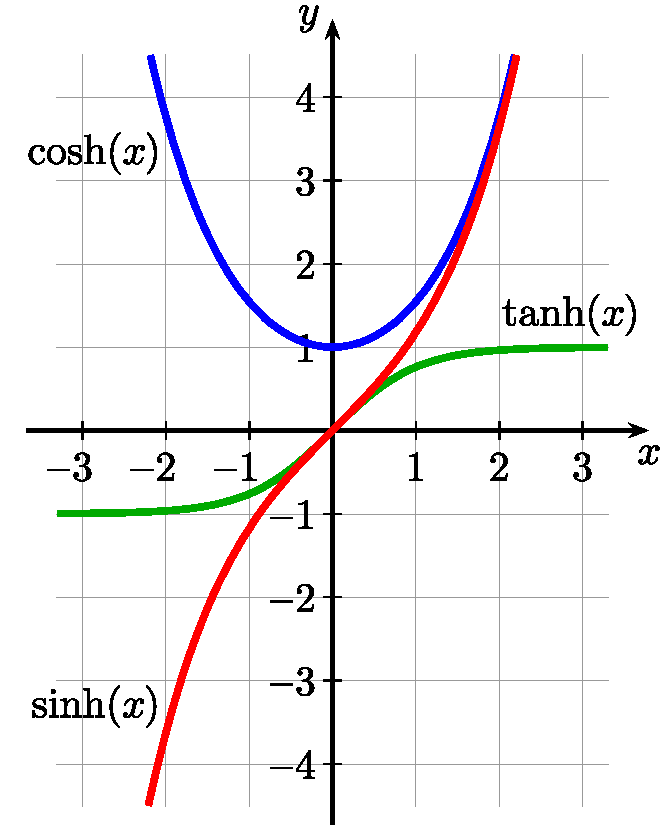
\includegraphics[width = 1.5cm]{./hyperbolis.pdf} 
	}
\end{sectionbox}

\begin{sectionbox}
	\subsection{Holomorphe (analytische, reguläre) Funktionen $\cx f$}
	Eine Funktion $\cx f$ ist \dots
	\begin{tablebox}{ll}
		holomorph & falls $\cx f$ in $G$ komplex differenzierbar ist.\\
		ganz & falls $\cx f$ in ganz $\C$ komplex differenzierbar ist.\\
		konform & falls Kurven Winkel- und Orientierungstreu bleiben.\\

	\end{tablebox}
	$\cx f$ ist genau dann holomorph, falls $\cx f(x+y\i) = u(x,y) + \i v(x,y)$ und
	\begin{itemize}\itemsep0pt
		\item $u,v$ sind stetig partiell diffbar
		\item Cauchy-Riemann DGLen sind erfüllt auf Gebiet $G$:\\
		$\partial_x u(x,y) = \partial_y v(x,y)$ \qquad $\partial_y u(x,y) = - \partial_x v(x,y)$
	\end{itemize}
	Holomorph: $\exp, \sin, \cosh$, Polynome, $\cx f\pm \cx g, \cx f \cx g, \frac{\cx f}{\cx g}, \cx f(\cx g),\cx f^{(n)}, \forall n\in \mathbb{N}$ \\
	\textbf{Mittelwerteigenschaft:} Ist $f:G\ra \C$ holomorph so ist der Wert $f(z_0)$ der Mittelwert der Funktionswerte auf dem Rand des Kreises mit dem Mittelpunkt $z_0$: \\
	$f(z_0)=\frac{1}{2\pi}\int_{0}^{2\pi}\cx f(z_0+r e^{it})\diff t$
\end{sectionbox}

\begin{sectionbox}
	\subsection{Harmonische Funktionen $u,v$}
	$u$ bzw. $v$ sind harmonisch, falls gilt:\\
	$\lpo u = \partial_{xx} u + \partial_{yy} u = 0$ \qquad\quad $\lpo v = \partial_{xx} v + \partial_{yy} v = 0$\\[0.5em]
	oder falls $\cx f(\cx z) = u + \i v$ holomorph ist; denn mit Satz von Schwarz:\\
	$\lpo u = \partial_{yx} v - \partial_{xy} v = 0$ \qquad\quad $\lpo v = - \partial_{yx} u + \partial_{xy} u = 0$
	\begin{cookbox}{Bestimmen der harmonischen Konjugierten}
			\item Geg: harm. Fkt. $u: G \ra \mathbb R, (x,y) \ra u(x,y)$
			\item Ges: harm. Fkt. $v: G \ra \mathbb R, (x,y) \ra v(x,y)$
			so, dass $f: G \ra \mathbb V, f(z) = u(x,y) + \i v (x,y)$
			\item $v(x,y) = \int u_x \diff y$ mit Integrationskonstante $g(x)$
			\item $v_x = -u_y \Ra g'(x)$
			\item $g(x) = \int g'(x) \diff x \Ra v$ bis auf Konstante $C$ bestimmt
			\item zugehörige holomorphe Fkt.
			$f (z) = u (x,y) + \i v(x,y)$
	\end{cookbox}
\end{sectionbox}

\begin{sectionbox}
%	\subsection{Möbiustransformation $\hat \C = \C \cup \eset{\infty}$}
	Einzige bijektive, holomorphe, konforme Abbildung von $\hat \C$ auf sich selbst.\\
	$\cx f:\C \setminus \eset{-\frac{d}{c}} \ra \C \setminus \eset{-\frac{d}{c}}, \cx f(\cx z) = \frac{a\cx z + b}{c\cx z + d}$ \qquad $ad - bc \ne 0$\\ 
	$\cx f^{-1}(\cx w) = \frac{d\cx w - b}{-c \cx w + a}$
\end{sectionbox}

\begin{sectionbox}
	\subsection{Komplexes Kurvenintegral}
	für $D \subset \mathbb C$ Gebiet, $f: D \ra \mathbb C$ stetig, $\cx \gamma: [t_1, t_2] \ra $ stetig diffbar Kurve
	\begin{cookbox}{Berechnen eines komplexen Kurvenintegrals}
		\item Bestimme Parametrisierung von $\cx \gamma$ \\
		$\cx \gamma = \cx \gamma_1 + \ldots + \cx \gamma_2$, $\cx \gamma_i : [a_i, b_i] \ra \C$
		\item Stelle Integrale auf \\
		$\int_{\cx \gamma_i} \cx f(\cx z) \diff \cx z = \int \limits_{a_i}^{b_i} \cx f\big(\cx \gamma_i(t)\big) \cdot \dot{\cx \gamma}_i (t) \diff t$\\
		Falls $\cx f$ holomorph: $\int_{\cx \gamma} \cx f(\cx z) \diff \cx z = \cx F\big(\cx \gamma(b)\big) - \cx F\big(\cx \gamma(a)\big)$
		\item Berechne die Integrale und addiere: \\
		$\int \limits_{\cx \gamma} \cx f(z\cx ) \diff \cx z = \sum \limits_{i = 1}^{h} \int_{\cx \gamma_i} \cx f(\cx z) \diff \cx z$
	\end{cookbox}
\end{sectionbox}

\begin{sectionbox}
	\subsection{Cauchy-Integralformel}
	Ist $\gamma$ eine geschlossene, doppelpunktfreie und positiv durchlaufene Kurve in einem einfach zusammenhängenden Gebiet $G$ und $f : G \ra \mathbb{C}$ holomorph, so gilt für jedes $z_0$ im Inneren von $\gamma$: \\
	\[\cx f(\cx z_0) = \frac{1}{2\pi \i} \ointctrclockwise_{\cx \gamma} \frac{\cx f(\cx z)}{\cx z - \cx z_0} \diff \cx z\]
	\begin{emphbox}\vspace{-5pt}
		\[\ointctrclockwise_{\cx \gamma} \frac{\cx f(\cx z)}{(\cx z - \cx z_0)^{k+1}} \diff \cx z = \frac{2\pi \i}{k!} \cx f^{(k)}\left(\cx z_0\right)\]
	\end{emphbox}
\end{sectionbox}

\begin{sectionbox}
	\subsection{Integralsatz von Cauchy}
	Falls keine Unstetigkeitsstelle innerhalb der Kurve $\cx \gamma$\\ 
	$\cx f: G \ra \C$ komplex diffbar auf offenem, einfach zusammenhängendem Gebiet $G \subset \C$. $\cx \gamma$ sei einfach geschlossene Kurve in $G$ (keine Doppelpunkte). \\
	$\oint \limits_{\cx \gamma} \cx f(\cx z) \diff \cx z = 0$
\end{sectionbox}

\begin{sectionbox}
	\subsection{Existenz einer Stammfunktion und Wegunabhängigkeit}
	Ist $\cx f: G \ra \C$ holomorph auf dem einfach zsh. Gebiet $G$, so existiert zu $\cx f$ eine Stammfunktion $\cx F$, und es gilt für jede in $G$ verlaufende Kurve $\cx \gamma$ mit Anfangspunkt $\cx \gamma(a)$ und Endpunkt $\cx \gamma(b)$: \\
	\begin{equation*}
		\int \limits_{\cx \gamma} \cx f(\cx z) \diff \cx z = \cx F(\cx \gamma (b)) - \cx F(\cx \gamma (a)) = \int\limits_a^bf(\gamma(t))\gamma'(t)dt
	\end{equation*}
\end{sectionbox}

\begin{sectionbox}
	\subsection{Singularitäten}
	Isolierte Singularität $\cx z_0\in G$: \quad $\cx f :G \setminus \eset{\cx z_0} \ra \C$ \ (einzelne Punkte, wo $f$ nicht definiert ist)
	\begin{itemize}
		\item Hebbare Singularität, falls $f$ auf punktierter Umgebung beschränkt ist.
		\item Pol $m$-ter Ordnung: $(\cx z - \cx z_0)^m \cx f(\cx z)$ ist hebbar in $\cx z_0$
		\item Wesentliche Singularität: Sonst.
	\end{itemize}
\end{sectionbox}

\begin{sectionbox}
	\subsection{Taylorreihe und Laurentreihe}
	\emph{Taylorreihe:} Falls $\cx f$ holomorph ist.
	\begin{equation*}
		\cx f(\cx z) = \sum\limits_{k = 0}^{\infty} \frac{\cx f^{(k)}\left(\cx z_0\right)}{k!} (\cx z - \cx z_0)^k
	\end{equation*}
	\emph{Laurentreihe:} Falls $\cx f$ nicht holomorph ist.\\
	\resizebox{\textwidth}{!}{
		% Nicht besonders schön, aber nur so lässt sich die Formel eigenständig und nicht inline darstellen.
		% Das Problem ist, dass die erste Summe in der Resize-Box im Inline-Modus dargestellt wird.
		\begin{minipage}{1.05\textwidth} 
		$$\cx f(z)=\sum_{k=- \infty}^{\infty} c_k (z-z_0)^{k} = \underbrace{\sum_{k=-\infty}^{-1} c_{k} (z-z_0)^{k}}_{\text{Hauptteil}} + \underbrace{\sum_{k=0}^{\infty} c_k (z-z_0)^{k}}_{\text{Nebenteil}}$$
		\end{minipage}
	}
	Konvergenz falls Hauptteil und Nebenteil konvergiert. \\ 
	Konvergenzradien: $R = \lim \abs{\frac{c_k}{c_{k+1}}} \in [0, \infty]$ \\ 
	Resiudensatz: $\Res_{z_0} \cx f = c_{-1} = \frac{1}{2\pi\i} \oint f(z) \diff z$
	
	\begin{emphbox}
		\raggedright
		$\Res_{\cx z_0} \frac{\cx g}{\cx h} = \frac{\cx g(\cx z_0)}{\cx h'(\cx z_0)}$ \qquad $\Res_{\cx z_0} \frac{\cx g(\cx z)}{(\cx z - \cx z_0)^m} = \frac{\cx g^{(m-1)}(\cx z_0)}{(m-1)!}$\\
		$\Res_{\cx z_0} \cx g \frac{\cx h'}{\cx h} = m \cx g(\cx z_0)$ \qquad $m:$ Ordnung der Polstelle
	\end{emphbox}
	\textbf{Allgemeiner Residuensatz} $f:G \setminus \eset{z_1, \ldots, z_n} \ra \mathbb C$ holomorph \\ 
	$\forall $ doppelpunktfrei, geschlossene und pos. orientierte Kurven $\gamma$ mit $z_1, \dots, z_n$ liegen im Inneren von $\gamma$:
	\begin{equation*}
		\oint_\gamma f(z) \diff z = 2 \pi \i \sum_{k=1}^{n} \Res_{z_k} f
	\end{equation*}
\end{sectionbox}

\begin{sectionbox}
	\begin{cookbox}{Bestimmen reeller Integrale mit dem Residuenkalkül}
		\item Reelles Integral $\int_{-\infty}^{\infty}\frac{p(x)}{q(x)}\diff x$
		\item Bestimme Singularitäten $z_1,\dots,z_n$ der komplexen Funktion $f(\cx z)=\frac{p(\cx z)}{q(\cx z)}$ in der oberen Halbebene, $\Im{ z_i}>0$
		\item Bestimme Residuen von $f(z)$ in den Singularitäten $z_1,\dots,z_n$
		\item $\int_{-\infty}^{\infty}\frac{p(x)}{q(x)}\diff x = 2 \pi \i \sum_{k=1}^{n} \Res_{z_k} f$
	\end{cookbox}
	\begin{cookbox}{Bestimmen reeller trigonometischer Integrale mit dem Residuenkalkül}
		\item Reelles Integral $\int_{-0}^{2\pi}R(\cos t, \sin t)\diff t$
		\item Substituiere $\frac{1}{2}(z+1/z)=\cos t$, $\frac{1}{2\i}(z-1/z)=\sin t$, $\frac{1}{\i z}\diff z=\diff t$
		\item Erhalte komplexe Fkt. $f(z)=R\left(\frac{1}{2}(z+1/z), \frac{1}{2\i}(z-1/z)\right)\frac{1}{\i z}$
		\item Bestimme Singularitäten $z_1,\dots,z_n$ der komplexen Funktion $f(\cx z)=\frac{p(\cx z)}{q(\cx z)}$ in des Einheitskreises $\abs{z}<1$
		\item Bestimme Residuen von $f(z)$ in den Singularitäten $z_1,\dots,z_n$
		\item $\int_{-0}^{2\pi}R(\cos t, \sin t)\diff t = 2 \pi \i \sum_{k=1}^{n} \Res_{z_k} f$
	\end{cookbox}
\end{sectionbox}

\begin{sectionbox}
	\subsection{Wichtige Taylorreihen}
	\begin{tablebox}{lll}
		$e^z$ & $\sum_{n=0}^\infty \frac{z^n}{n!}$ & $\forall z \in \mathbb{C}$ \\
		$\ln(z)$ & $\sum_{n=1}^\infty \frac{(-1)^{n+1}}{n}(z-1)^n$ & $0<z\le2$ \\ [0.5em]
		$\frac{1}{1-z}$ & $\sum^\infty_{n=0} z^n$ & $\abs{z} < 1$ \\
		$\sin z$ & $\sum^{\infty}_{n=0} \frac{(-1)^n}{(2n+1)!} z^{2n+1}$ & $\forall  z \in \mathbb{C}$ \\[0.7em]
		$\cos z$ & $\sum^{\infty}_{n=0} \frac{(-1)^n}{(2n)!} z^{2n}$ & $\forall  z \in \mathbb{C}$ \\[0.7em]
		$\sinh z$ & $\sum^{\infty}_{n=0} \frac{z^{2n+1}}{(2n+1)!}$ & $\forall  z \in \mathbb{C}$ \\[0.7em]
		$\cosh z$ & $\sum^{\infty}_{n=0} \frac{z^{2n}}{(2n)!}$ & $\forall  z \in \mathbb{C}$ \\

	\end{tablebox}
	
\end{sectionbox}


% SECTION ======================================================================
\section{Partielle Differentialgleichungen 1. Ordnung}
% ==============================================================================

\begin{sectionbox}
	\subsection{Lineare pDGLen 1. Ordnung mit konstanten Koeffizienten}
	Geg.: $a u_x+b u_y =f(x,y)$ mit $a \neq 0 \neq b$, ges.: $u=u(x,y)$
	\begin{cookbox}{Lösen einer linearen pDGL 1. Ordnung mit konstanten Koeffizienten}
		\item Substitution: $r=r(x,y)=bx+ay$ und $s=s(x,y)=bx-ay$
		\item $U(r,s) = u(\frac{r+s}{2b},\frac{r-s}{2a}) = u(x,y)$  und \\ $F(r,s) = f(\frac{r+s}{2b},\frac{r-s}{2a}) = f(x,y)$
		\item Einsetzen liefert $U_{r}=\frac{1}{2ab}F(r,s) $
		\item Lösung U: $\; \; U(r,s)=\int \frac{1}{2ab} F(r,s)\diff r+G(s)$ mit diff'barem $G(s)$
		\item Rücksubstitution liefert $u(x,y)$
		\item Anfangsbedingung z.B. $u(x,0) = g(x)$ legt $G(s)$ fest
	\end{cookbox}
\end{sectionbox}

\begin{sectionbox}
	\subsection{Lineare pDGL 1. Ordnung}
	Geg.: $a(x,y)u_x+b(x,y)u_y=0$, ges.: $u=u(x,y)$
	\begin{cookbox}{Lösen einer linearen homogenen pDGL 1. Ordnung (2 Variablen)}
		\item $\frac{\diff y}{\diff x}=\frac{b(x,y)}{a(x,y)}$ (ist gDGL), alternativ $\frac{\diff x}{\diff y}=\frac{a(x,y)}{b(x,y)}$ 
		\item Löse gDGL und erhalte $y=y(x)=F(x,c) $
		\item Löse die Gleichung $y(x)=F(x,c)$ nach $c = c(x,y)$ auf (falls möglich)
		\item $u(x,y)=f(c(x,y))$ ist für jede stetig diff'bare Fkt. $f$ eine Lösung der pDGL
		\item $f$ wird durch evtl. gegebene Anfangsbedingung festgelegt
	\end{cookbox}
	\label{subsubsec:linpdgl}
	Geg.: $a(x,y,z)u_x+b(x,y,z)u_y+c(x,y,z)u_z=0$, ges.: $u=u(x,y,z)$
	\begin{cookbox}{Lösen einer linearen homogenen pDGL 1. Ordnung (3 Variablen)}
		\item $\frac{\diff y}{\diff x}=\frac{b(x,y,z)}{a(x,y,z)}$ und $\frac{\diff z}{\diff x}=\frac{c(x,y,z)}{a(x,y,z)}$ (ist ein System von gDGL), \\
			alternativ $\frac{\diff x}{\diff y}$, $\frac{\diff z}{\diff y}$ oder $\frac{\diff x}{\diff z}$, $\frac{\diff y}{\diff z}$
		\item Löse das System von gDGLen und erhalte \\$y=y(x)=F(c_{1},x) $ und $z=z(x)=G(c_{2},x) $
		\item Löse das System $y(x)=F(c_{1},x) $ und $z(x)=G(c_{2},x) $ nach $c_{1}=c_{1}(x,y,z) $ und $c_{2}=c_{2}(x,y,z) $ auf (falls möglich)
		\item $ u(x,y,z)=f(c_{1}(x,y,z),c_{2}(x,y,z))$ ist für jede stetig diff'bare Fkt. $f$ eine Lösung der pDGL
		\item $f $ wird durch evtl. gegebene Anfangsbedingung festgelegt
	\end{cookbox}
\end{sectionbox}

\begin{sectionbox}
	\subsection{Quasilineare pDGL 1. Ordnung}
	Geg.: $a(x,y,u)u_x+b(x,y,u)u_y=c(x,y,u)$, ges.: $u=u(x,y)$ \\ \vspace{-1em}
	\begin{cookbox}{Lösen einer quasilinearen pDGL 1. Ordnung}
		\item Betrachte lineare pDGL in drei Variablen $x,y,u$:
		\\$a(x,y,u)F_{x}+b(x,y,u)F_{y}+c(x,y,u)F_{u}=0$
		\item Löse lineare pDGL mit Ansatz aus {\bf\ref{subsubsec:linpdgl}} und erhalte	$F=F(x,y,u) $
		\item Durch $F(x,y,u)=0 $ ist implizit eine Lösung $u=u(x,y) $ gegeben
	\end{cookbox}
	AWP gegeben $u(p(x),q(x))=r(x)$, z.B. $u(x,0)=x$
	\begin{cookbox}{Lösen einer quasilinearen pDGL 1. Ord. mit dem Charakteristikverfahren}
		\item Ansatz: $v(s)=u(x(s),y(s))$ \qquad ($u$ hängt nur von einer Variable $s$ ab)
		\item Ableiten des Ansatzes nach $s$ (Kettenregel): \quad $\dot v = u_x \dot x + u_y \dot y$
		\item Vergleichen mit pDGL liefert DGL-System:\\ 
		 $\dot x =a(x,y,u) \qquad \dot y=b(x,y,u) \qquad \dot v=c(x,y,u)$
		\item Setze $s=0$ in Ansatz $v(s)$: \quad $v(0)=u(x(0),y(0))$ mit $x=x_0$
		\item Vergleichen mit AWP der pDGL liefert AWP für DGL-System: \\
		$x(0)=p(x_0) \qquad y(0)=q(x_0) \qquad v(0)=r(x_0)$ 
		\item Löse DGL-System und erhalte $v(s)$
		\item Bestimme $s=f(x,y)$ und $x_0=g(x,y)$ und mit Rücksub. $u(x,y)$
	\end{cookbox}
\end{sectionbox}


% SECTION ======================================================================
\section{Partielle Differentialgleichungen 2. Ordnung}
% ==============================================================================
%\begin{sectionbox}
%	\subsection{Typeneinteilung von pDGLen 2. Ordnung mit zwei Variablen}
%%	Gesucht: $u=u(x,y)$ \\
%	Gegeben: $a(x,y)u_{xx}+2b(x,y)u_{xy}+c(x,y)u_{yy}+d(x,y)u_{x}+e(x,y)u_{y}+f(x,y)u=g(x,y)$\\
%	$\Ra$ Hauptteil: $a(x,y)u_{xx}+2b(x,y)u_{xy}+c(x,y)u_{yy}$ \\ \\
%	Die pDGL ist auf $D\subseteq \mathbb{R}^2$ \dots
%	\begin{tablebox}{ll}
%		elliptisch & falls $a(x,y)c(x,y)-b(x,y)^2>0 $ für alle $(x,y) \in D $ \\
%		parabolisch & falls $a(x,y)c(x,y)-b(x,y)^2=0 $ für alle $(x,y) \in D $ \\
%		hyperbolisch & falls $a(x,y)c(x,y)-b(x,y)^2<0 $ für alle $(x,y) \in D $ \\
%		gemischter Typ & falls verschiedene $(x,y) \in D $ versch. Eigenschaften aufweisen
%	\end{tablebox}
%\end{sectionbox}

\begin{sectionbox}
	\subsection{Lösungsmethode}
	\label{subsubsec:separationsansatz}
	\begin{cookbox}{Lösen der pDGL mit dem Separationsansatz}
		\item Setze $u(x,y)=f(x)g(y) $ in die pDGL ein und erhalte zwei gDGLen für $f$ und $g$. (Faktor $k$ nicht vergessen!)
		\item Löse die zwei gDGLen und erhalte $f=f(x)$ und $g=g(y) $
		\item Eine Lösung der pDGL ist $u(x,y)=f(x)g(y) $
	\end{cookbox}
\end{sectionbox}

% SECTION ======================================================================
\section{Laplace- und Poissongleichung \quad $-\laplace u = f$}
% ==============================================================================

%Folgender Abschnitt wurde aufgrund von Platzmangel weggelassen

%\begin{sectionbox}
%	\subsection{Randwertprobleme (RWP) für Poissongleichung}
%	\begin{flushleft}
%	Geg.: $-\laplace u = f$ und ein RWP. Ges.: $u=u(x,y)$ oder $u=u(x,y,z)$
%	\end{flushleft}
%	\begin{tablebox}{p{\textwidth}}
%		\textbf{Dirichlet RWP}\\
%		$-\laplace u(\vec x)=f(\vec x) $ für alle $x \in D $ und $u(\vec x)=u_{0}(\vec x) $ für alle $x \in \partial D$ \\
%		\textbf{Neumann RWP}\\
%		$-\laplace u(\vec x)=f(\vec x) $ für alle $x \in D $ und $\frac{\partial u}{\partial \vec n}(\vec x)=u_{0}(\vec x) $ für alle $x \in \partial D $ \\
%		\textbf{Gemischtes RWP} \\
%		$-\laplace u(\vec x)=f(\vec x) $ für alle $x \in D $ und $\frac{\partial u}{\partial \vec n}(\vec x)+k(\vec x)u(\vec x)=u_{0}(\vec x) $ für alle $x \in \partial D $ \\
%	\end{tablebox}
%	wobei $\vec n$ = Normaleneinheitsvektor, der aus D hinausweist und $k=k(\vec x)$ ist eine stetige Funktion.
%	\begin{tablebox}{lp{0.8\textwidth}}
%		Inneres RWP & falls $D$ ein beschränktes Gebiet \\
%		Äußeres RWP & falls $D$ Komplement eines beschränkten Gebietes ist (Dann sind weitere Randwertbedingungen an die Lösungen zu stellen)
%	\end{tablebox}
%\end{sectionbox}
	
\begin{sectionbox}
	\subsection{Laplacegleichung \quad $-\laplace u=0$}
	\subsubsection{Allgemeine Lösung der Laplacegleichung}
	\resizebox{\textwidth}{!}{
		$u(r,\varphi)=
		\begin{cases}
		u_{n}(r,\varphi)=(a_{n}\cos(n \varphi)+b_{n}\sin(n \varphi))r^{n} & \text{für } n \in \mathbb{Z}\setminus\{0\}
		\\
		a+b \; \ln(r) & \text{für } n=0
		\end{cases}$
	}
	für beliebige $a_{n},b_{n} \in \mathbb{R}$ bzw. $a,b \in \mathbb{R}$.
	\subsubsection{Dirichlet'sches RWP für einen Kreis}
	Geg.: $-\laplace u(x,y)=0$ für $x^2+y^2<R^2$ und $u(x,y)=u_0(x,y)$ für $x^2+y^2=R^2$
	\begin{cookbox}{Lösen eines Dirichlet'schen RWP für einen Kreis}
		\item Bestimme die Koeffizienten $a_n$ und $b_n$ der Fourierreihe der $2\pi$-periodischen Funktion $u_0(\varphi):[0,2\pi)\ra \R$
		\item Erhalte die Lösung $u=u(r,\varphi)$ als Reihendarstellung in Polarkoordinaten:\\
		$u(r,\varphi)=\frac{a_0}{2}+\sum_{k=1}^{\infty}\bigl(a_k \cos(k\varphi)+b_k \sin(k\varphi)\bigr)\big(\frac{r}{R}\big)^k$
		\item Falls AWP gegeben als $x^2+y^2>R^2$, wird $r$ und $R$ vertauscht:\\
		$u(r,\varphi)=\frac{a_0}{2}+\sum_{k=1}^{\infty}\bigl(a_k \cos(k\varphi)+b_k \sin(k\varphi)\bigr)\big(\frac{R}{r}\big)^k$
		\item Umformen von $u(r,\varphi)$ mit $x=r\cos\varphi$, $y=r\sin\varphi$ ergibt $u(x,y)$
	\end{cookbox}
	\subsubsection{Dirichlet'sches RWP für ein Quadrat}
	Geg.: $-\laplace u(x,y)=0$ auf dem Quadrat $D=[0,a]^2$ mit definierten Randwerten $u(x,0)$, $u(x,a)$, $u(0,y)$ und $u(a,y)$ für $x,y\in [0,a]$
	% Geg.: $-\laplace u(x,y)=0$ auf dem Quadrat $D=[0,a]^2$ mit den Randwerten $u(x,0)=f_1(x)$, $u(x,1)=f_2(x)$, $u(0,y)=f_3(y)$ und $u(1,y)=f_4(y)$ für $x,y\in [0,a]$
	\begin{cookbox}{Lösen eines Dirichlet'schen RWP mit dem Separationsansatz}
		\item Ansatz $u(x,y)=f(x)g(y)$ aus {\bf\ref{subsubsec:separationsansatz}} liefert: $\frac{f''}{f}=k$ und $\frac{g''}{g}=-k$
		\item Lösen der gDGLen 2. Ordnung liefert:\\
		$f(x)=\begin{cases}
		c_1e^{\sqrt{k}x}+c_2e^{-\sqrt{k}x} & \text{für } k>0\\
		c_1+c_2x & \text{für }  k=0\\
		c_1\cos\sqrt{-k}x+c_2\sin\sqrt{-k}x & \text{für } k<0
		\end{cases}$ \qquad und \\
		$g(y)=\begin{cases}
		d_1\cos\sqrt{k}y+d_2\sin\sqrt{k}y & \text{für } k>0\\
		d_1+d_2y & \text{für }  k=0\\
		d_1e^{\sqrt{-k}y}+d_2e^{-\sqrt{-k}y} & \text{für } k<0
		\end{cases}$
		\item Vorgegebene Randwerte definieren die Lösung des RWP $u(x,y)=f(x)g(y)$ durch die Konstanten $k,c_1,c_2,d_1,d_2\in\R$
	\end{cookbox}
\end{sectionbox}

% SECTION ======================================================================
\section{Wärmeleitungsgleichung \quad \(u_{t}=c^{2} \laplace{u}\)}
% ==============================================================================

\begin{sectionbox}
	\(u_{t}=c^{2}u_{xx}\) für \(x \in (0,l), t\geq 0\) \\
	Geg: \(u(x,0)=g(x)\) und \(u(0,t)=u(l,t)=0\) und Länge \(l\) und \(c=\mathrm{const}>0\)
	\begin{cookbox}{Lösen eines Nullrandproblems für einen Stab}
		\item Bestimme Koeffizienten \(b_{n}\) von \(g(x)\): \\
		\(b_{n}=\frac{2}{l} \int_{0}^{l} g(x)\sin\left(n\frac{\pi}{l}x\right)dx\) \qquad für \(n=1,2,3,4,... \)
		\item Lösung \(u(x,t)\) als Reihendarstellung: \vspace{-5pt}		 % Platz sparen wo nur geht
		\[u(x,t)=\sum_{n=1}^{\infty} b_{n} \exp\left(-c^{2}\left(\frac{n\pi}{l}\right)^{2}t\right)\sin\left(n\frac{\pi}{l}x\right)\]
	\end{cookbox}
	\(u_{t}=c^{2}u_{xx}\) für \(x \in (0,l), t\geq 0\) \\
	Geg: \(u(x,0)=g(x)\) und \(u_x(0,t)=u_x(l,t)=0\)
	\begin{cookbox}{Lösen eines modifizierten Nullrandproblems für einen Stab}
		\item Bestimme Koeffizienten \(a_{n}\) von \(g(x)\): \\
		\(a_{n}=\frac{2}{l} \int_{0}^{l} g(x)\cos\left(n\frac{\pi}{l}x\right)dx\) \qquad für \(n=0,1,2,3,... \)
		\item Lösung \(u(x,t)\) als Reihendarstellung: \vspace{-5pt}		 % Platz sparen wo nur geht
		\[u(x,t)=\frac{a_0}{2} + \sum_{n=1}^{\infty} a_{n} \exp\left(-c^{2}\left(\frac{n\pi}{l}\right)^{2}t\right)\cos\left(n\frac{\pi}{l}x\right)\]
	\end{cookbox}
\end{sectionbox}

% SECTION ======================================================================
\section{Wellengleichung \quad \(u_{tt}=c^{2} \laplace{u} \)}
% ==============================================================================
\begin{sectionbox}
\(u_{tt}-c^{2} u_{xx}=0\) \\
Geg: \(l\) = Länge der Saite und \(u(x,0)=g(x), u_{t}(x,0)=v(x), u(0,t)=u(l,t)=0\) und \(c=\mathrm{const}>0 \)
\begin{cookbox}{Lösung eines Anfangs-Randwertproblems für eine schwingende Saite}
\item Bestimme Koeffizienten \(a_{n}\) von \(g(x)\) und \(b_{n}\) von \(v(x)\): \\
\(a_{n}=\frac{2}{l}\int_0^l  g(x)\sin\left(n\frac{\pi}{l}x\right)dx\) \qquad für \(n=1,2,3,4,... \)\\
\(b_{n}=\frac{2}{n\pi c} \int_0^l  v(x)\sin\left(n\frac{\pi}{l}x\right)dx\) \qquad für \(n=1,2,3,4,... \)
\item Lösung \(u(x,t)\) als Reihendarstellung: \vspace{-5pt}		 								% Platz sparen wo nur geht
\[u\left(x,t\right)= \sum_{n=1}^{\infty} \sin\left(\frac{n \pi}{l}x\right)\left(a_{n}\cos\left(c\frac{n\pi}{l}t\right)+b_{n}\sin\left(c\frac{n\pi}{l}t\right)\right)\]
\end{cookbox}
\end{sectionbox}
% Roberto Ende

\vspace{-1cm} 							% Löst Problem mit Seitenzahlen in der Fußzeile

% Dokumentende
% ======================================================================
\end{document}
